\chapter{Arithmetic, Logic, and Condition State}
\label{ch:arithmetic-condition}

At fixed width, addition produces a stored word even when the mathematical
sum lies outside the word's unsigned or signed range. Carry and signed
overflow describe different facts about that event. Confusing them is easy;
making both rules explicit is easier.

Arithmetic also changes more than numbers. One machine writes condition bits
that a later branch can read. Another writes only a destination register and
asks a branch to compare registers directly. A third can materialize a Boolean
answer as an ordinary word. The calculation and the place where its facts are
recorded must both enter the proof.

\begin{keyidea}[title={A result word does not contain every arithmetic fact}]
The low \(w\) bits determine the stored result. They do not by themselves say
whether the unsigned sum crossed \(2^w\), whether the signed sum left its
range, or which condition state an instruction promised to update. Those are
separate parts of the transition.
\end{keyidea}

\section{Why machines record arithmetic conditions}

A program rarely computes only to keep the result. It also asks whether the
result was zero, whether one value was less than another, whether an unsigned
addition carried, or whether a signed calculation left its representable
range. Early arithmetic units exposed some of these facts as condition state
because the next instruction could branch on them without storing another
ordinary word.

That design remains visible in x86-64. Selected arithmetic and compare forms
write named status flags, and later conditional instructions read Boolean
formulas over those flags. RISC-V's base integer design usually keeps the
condition in the instruction that needs it or writes an explicit zero-or-one
comparison result. A0 uses four condition bits so that the hidden-state style
can be printed in full before we compare it with the alternatives.

Neither state shape is intrinsically more semantic. A flag is architectural
state if later instructions can observe it. A Boolean register is ordinary
state with a convention about its value. A direct branch comparison can avoid
materializing either. What matters is whether the surrounding program receives
the information it needs.

\begin{archive}[title={Condition state is a compact memory of a calculation}]
A condition code preserves selected facts while discarding the operands and,
for a compare instruction, often the arithmetic result itself. It is a small
summary of a larger event. The summary is useful precisely because it is
incomplete; proofs must therefore say which later questions it can answer.
\end{archive}

\section{One addition, four separate questions}

Let \(x\) and \(y\) be width-\(w\) words. Their ordinary nonnegative readings
lie from zero through \(2^w-1\). Write
\[
  s=\langle x\rangle_u+\langle y\rangle_u
\]
for the mathematical unsigned sum and
\[
  r=s\bmod 2^w
\]
for the stored word. Four questions now have distinct answers:

\begin{enumerate}
\item What is the stored result \(r\)?
\item Is \(r\) zero?
\item Is the high bit of \(r\) one?
\item Did the unsigned or signed mathematical reading leave its range?
\end{enumerate}

A0 names the corresponding bits \(Z,N,C,V\). Zero and negative depend only on
the stored result:
\[
 Z\quad\hbox{iff}\quad r=0,
 \qquad
 N=\mathrm{bit}_{w-1}(r).
\]
Carry records an unsigned boundary:
\[
 C\quad\hbox{iff}\quad s\geq 2^w.
\]
Signed overflow records a signed boundary. It holds exactly when the operands
have the same high bit and the result has the other high bit.

\begin{figure}[htbp]
\centering
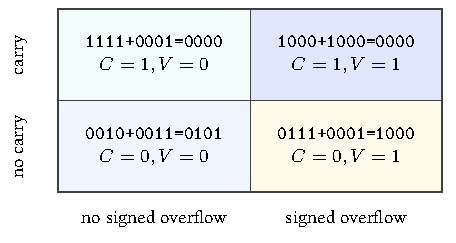
\includegraphics[width=0.83\textwidth]{figures/carry-overflow-quadrants}
\caption{Width-four addition supplies examples in all four carry and signed-
overflow combinations. Neither condition implies the other.}
\figalt{A two-by-two grid gives four-bit additions for no carry no overflow, no carry overflow, carry no overflow, and carry overflow.}
\label{fig:carry-overflow-quadrants}
\end{figure}

The upper-left example in the figure adds \code{1111} and \code{0001}. The
unsigned readings are 15 and 1, so the mathematical sum reaches 16 and sets
carry. The signed readings are -1 and 1, whose sum is representable, so signed
overflow is clear. The lower-right example adds 7 and 1. It has no unsigned
carry, but the signed result 8 is outside the width-four signed range and sets
overflow.

\subsection{The widened identity separates storage from range}

Because two unsigned width-\(w\) readings sum to at most \(2^{w+1}-2\), one
extra bit is enough to hold their exact sum. There are unique values
\(C\in\{0,1\}\) and \(0\leq r<2^w\) such that
\[
  \langle x\rangle_u+\langle y\rangle_u=C2^w+r.
\]
The low part \(r\) is the stored word. The coefficient \(C\) is the carry.
No approximation or particular circuit is involved. The equation is Euclidean
division by \(2^w\).

\begin{figure}[htbp]
\centering
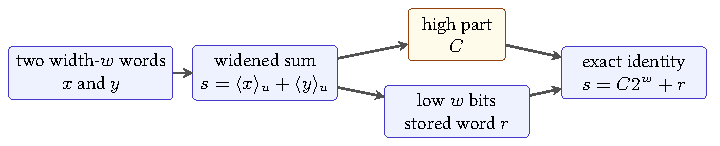
\includegraphics[width=0.94\textwidth]{figures/extended-addition-decomposition}
\caption{Widening makes the unsigned arithmetic exact. Truncation stores the
low word, while the high bit records whether the unsigned range was crossed.}
\figalt{Two width-w inputs form a widened sum, which splits into one carry bit and a low width-w stored word satisfying the exact decomposition.}
\label{fig:extended-addition-decomposition}
\end{figure}

The identity gives two interchangeable definitions:
\[
  r=s\bmod 2^w,
  \qquad
  C=1\quad\hbox{iff}\quad s\geq 2^w.
\]
It also yields a useful test that avoids a wider host type. For width-\(w\)
unsigned addition, carry occurs exactly when the stored result is below either
operand. If no carry occurs, \(r=x+y\) is at least each operand. If carry
occurs, subtracting \(2^w\) makes \(r\) smaller than each positive
contributor. A proof assistant or solver can check this equivalence directly
over bit vectors.

The stored word has another algebraic meaning. Width-\(w\) words under
addition form arithmetic modulo \(2^w\). Addition is associative and has
zero as an identity even when intermediate mathematical sums cross the
unsigned boundary. Carry is not part of that modular result; it is extra
information about the chosen unsigned representatives. This distinction lets
one theorem establish a modular calculation while another establishes that no
range boundary was crossed.

\begin{example}[title={One result, two claims}]
At width eight, \code{FA + 0A} stores \code{04}. The modular equation
\(250+10\equiv4\pmod{256}\) holds without a precondition. The ordinary
integer equation \(250+10=4\) is false, while the widened identity
\(250+10=1(256)+4\) is exact. A result theorem must say which of these
meanings it promises.
\end{example}

\begin{warning}[title={Say which overflow you mean}]
The word \emph{overflow} is incomplete in a fixed-width claim. Unsigned carry
and signed overflow answer different range questions and can disagree. Name
the reading, range, and condition bit.
\end{warning}

\subsection{Zero and negative are readings of the stored word}

The zero condition has no signedness ambiguity. A width-\(w\) word has
unsigned reading zero exactly when all bits are zero, and its signed reading is
then also zero. Thus \(Z\) can support equality-to-zero tests for either
reading. What produced the word is irrelevant once the instruction policy says
that \(Z\) is defined from its result.

The negative condition is different. \(N\) copies the high bit, so it says
that the stored word has a negative two's-complement reading. It does not say
that an unsigned result is below zero, and it does not by itself say that a
signed mathematical calculation produced a negative value. If signed
overflow occurred, the stored signed reading has wrapped away from the
mathematical result.

These facts explain several branch formulas. After a subtraction that does not
overflow, \(N\) alone agrees with signed less-than. Without that premise,
\(N\ne V\) repairs the wrapped cases. Equality uses \(Z\) without a range
premise. Unsigned order uses the borrow convention rather than \(N\), because
the high bit is simply part of the unsigned magnitude.

\begin{proofkit}[title={Zero after subtraction means equal words}]
Modular subtraction stores zero exactly when
\(x-y\equiv0\pmod{2^w}\). Both unsigned readings lie in an interval of
length \(2^w\), so their difference lies strictly between \(-2^w\) and
\(2^w\). The only multiple of \(2^w\) in that range is zero. Therefore the
readings, and hence the words, are equal. The reverse direction is immediate.
\end{proofkit}

Condition names still need an instruction policy. A move might leave \(Z\)
unchanged even when it writes a zero word; a logic instruction might define
\(Z\) from its result; a compare might define \(Z\) from a subtraction it
does not store. The mathematical predicate and the architectural decision to
record it are separate claims.

\section{Deriving the signed-overflow rule}

The sign rule is not a hardware incantation. It follows from the signed range.
If one operand is nonnegative and the other negative, their sum lies between
them. It cannot exceed both ends of the representable interval. Therefore
opposite-sign addition cannot overflow.

If both operands are nonnegative, signed overflow occurs exactly when the
mathematical sum is at least \(2^{w-1}\). The stored high bit is then one, so
the result appears negative. If both operands are negative, their sum can fall
below \(-2^{w-1}\). Modular reduction then yields a stored word whose high bit
is zero. These are precisely the same-input-sign, different-result-sign cases.

Writing \(h(z)\) for the high bit of word \(z\), the rule is
\[
  V=\neg(h(x)\mathbin{\mathsf{xor}}h(y))
      \mathbin{\mathsf{and}}
      (h(x)\mathbin{\mathsf{xor}}h(r)).
\]

\begin{proofkit}[title={A reader proof of addition overflow}]
Split on whether the two input high bits agree. When they differ, one signed
operand is nonnegative and the other negative, so the sum stays within range.
When both are zero, overflow means the nonnegative sum reaches the signed upper
boundary, which makes the stored high bit one. When both are one, overflow
means the negative sum crosses the signed lower boundary, which makes the
stored high bit zero. These cases match the Boolean formula.
\end{proofkit}

This proof handles every width \(w>0\). Exhausting all 256 pairs at width four
is still useful, but it checks an instance. The case argument explains why the
same rule holds at width 8, 32, 64, or another positive width.

The boundary cases are worth naming. Adding one to the greatest signed
positive word sets \(V\) and produces the least signed word. Adding negative
one to the least signed word may set carry while clearing \(V\), because the
signed sum remains representable. Adding the two least signed words sets both
conditions at widths above one. These examples defeat the vague rule that
overflow means the high bit changed: many legitimate sums change the high bit,
and some overflowing sums wrap to a word with the same high bit as one
operand.

\section{Subtraction, borrow, and comparison}

Subtraction stores
\[
  r=x-y\bmod 2^w.
\]
A0 defines \(C\) as \emph{no unsigned borrow}: it is one exactly when the
unsigned reading of \(x\) is at least that of \(y\). This polarity must be
printed because other conventions may name or invert the condition differently.

At width four, \code{0011-0101} stores \code{1110}. Since unsigned 3 is below
5, a borrow was needed and A0 clears \(C\). Conversely,
\code{0101-0011} stores \code{0010} and sets \(C\). In both cases, \(Z\) and
\(N\) come from the stored result.

Signed subtraction overflows exactly when the input signs differ and the
result sign differs from the minuend's sign. Subtracting a negative number
from a nonnegative one can become too positive. Subtracting a nonnegative
number from a negative one can become too negative. Same-sign subtraction
cannot cross a signed boundary in that way.

A0's \code{cmp rs1,rs2} performs the subtraction condition calculation without
writing the result to an ordinary register. Its later signed less-than predicate
is \(N\ne V\). Its unsigned lower-than predicate is \(\neg C\). Equality is
\(Z\). These formulas recover comparisons from the retained summary.

\begin{example}[title={Why the sign bit alone is not signed less-than}]
At width four, compare \code{0111} with \code{1111}. The signed readings are 7
and -1, so 7 is not less. The stored subtraction is
\code{0111-1111=1000}, whose high bit sets \(N\). Signed overflow also sets
\(V\), so \(N\ne V\) is false. Reading \(N\) alone would give the wrong answer.
\end{example}

The correction by \(V\) is the compact trace of wraparound. When signed
subtraction stays in range, the result sign tells the ordering. When it
overflows, that sign is reversed from the mathematical ordering, and the
overflow bit reverses the decision back.

\subsection{Subtraction can be read three ways}

The same stored subtraction supports three claims. As a word equation,
\[
  r\equiv x-y\pmod{2^w}
\]
always holds. As an unsigned natural subtraction, \(r=x-y\) holds without
wrap exactly when \(\langle x\rangle_u\geq\langle y\rangle_u\). As a signed
integer subtraction, the stored signed reading equals the mathematical
difference exactly when \(V=0\). A theorem that promises correct subtraction
must choose among these meanings.

Subtraction may also be implemented algebraically as addition of a two's-
complement inverse:
\[
  x-y\equiv x+(\mathord{\sim}y)+1\pmod{2^w}.
\]
This identity explains why an arithmetic unit can reuse addition machinery,
but it does not settle flag polarity. The final carry-out of this addition is
one exactly when no unsigned borrow is needed under A0's convention. An ISA
that defines a borrow flag with the opposite polarity must invert that fact at
its architectural boundary.

\begin{proofkit}[title={Unsigned comparison from subtraction}]
Let \(a=\langle x\rangle_u\) and \(b=\langle y\rangle_u\). If \(a\geq b\),
the ordinary difference lies in \([0,2^w-1]\), so modular reduction changes
nothing and A0 sets no-borrow \(C\). If \(a<b\), the negative difference is
represented by adding \(2^w\), which is precisely the wrap associated with a
borrow, and A0 clears \(C\). Thus \(\neg C\) is equivalent to unsigned
less-than and \(C\) to unsigned greater-than-or-equal.
\end{proofkit}

Equality needs less retained information. Modular subtraction stores zero
exactly when the two width-\(w\) words are identical, so \(Z\) recovers word
equality without a signedness choice. Signed and unsigned order disagree on
some pairs, but equality does not: both readings are one-to-one over the same
finite set of words.

Negation reveals a special signed boundary. The least signed word represents
\(-2^{w-1}\). Its mathematical negation \(2^{w-1}\) is not representable, so
modular negation returns the same word and sets signed overflow under a policy
that reports it. Every other signed word has a representable negation. This is
why an absolute-value routine needs an explicit policy for the least signed
input.

\begin{example}[title={One subtraction, two orderings}]
At width eight, compare \code{FF} with \code{01}. Unsigned 255 is greater
than 1, so no borrow is needed and \(C=1\). Signed -1 is less than 1, and the
signed predicate \(N\ne V\) is true. The same subtraction summary answers
both questions because the branch chooses a different formula.
\end{example}

\section{Logic and shifts need condition policies too}

A0's AND, OR, XOR, and NOT instructions set \(Z\) and \(N\) from the result
and clear \(C\) and \(V\). The clearing is a policy, not a theorem about
Boolean algebra. Another ISA may preserve, clear, define, or leave selected
condition bits undefined for a corresponding operation.

The distinction matters after a sequence. Suppose an addition sets carry, a
logical operation produces the same destination in two candidate programs,
and a later branch reads carry. If one logical semantics clears carry while
another preserves it, destination-only tests miss the difference.

Shifts add a further question: which bit was last shifted out? A0 uses the low
unsigned value of \(rs2\) modulo \(w\) as the count. A zero-count shift
preserves the source result and clears \(C\). A nonzero shift writes the last
bit removed into \(C\), sets \(Z,N\), and clears \(V\).

For width eight, shifting \code{10110001} left by three produces
\code{10001000}. The last bit removed is the original bit 5, which is one, so
\(C=1\). Logical right shift fills from the high side with zeros. Arithmetic
right shift repeats the original high bit. The two right shifts agree for a
source high bit of zero and can differ when it is one.

\begin{tryit}[title={Follow the bit that becomes carry}]
Write the source bits above positions 7 through 0. For left shifts by 1, 2,
and 7, circle the last bit that leaves the word. Repeat for logical right
shifts. Then test count zero separately; do not infer its condition rule from
a diagram showing movement.
\end{tryit}

Large and zero shift counts are frequent semantic fault lines. A0's modulo-
width rule is part of its model. RV64I and x86-64 selected forms have their own
count rules. A cross-ISA theorem must either relate those rules on a restricted
domain or expose the difference.

\subsection{A shift theorem needs a count domain}

For a logical left shift by a mathematical count \(k\) with
\(0\leq k<w\), the stored result has unsigned reading
\[
  (\langle x\rangle_u2^k)\bmod 2^w.
\]
For a logical right shift in the same count range, its reading is
\[
  \left\lfloor\frac{\langle x\rangle_u}{2^k}\right\rfloor.
\]
These clean formulas do not define what happens for \(k=w\), larger counts,
or a negative mathematical count. The instruction semantics must first map
its encoded or register-supplied count into an effective count domain.

A0 chooses the low unsigned count modulo \(w\). At width eight, raw counts
0, 8, and 16 therefore all have effective count zero. A theorem restricted to
raw counts below eight can use the simple formulas directly. A theorem over
every input word must include the modulo operation. Confusing raw and
effective counts is especially dangerous in cross-ISA work because two
machines can agree on small counts and diverge exactly at the boundary.

Arithmetic right shift needs a signed reading. For an effective count below
the width, it behaves like division by \(2^k\) rounded toward negative
infinity under the usual sign-extension rule. That rounding matters:
arithmetic shift of -3 by one produces -2, whereas integer division specified
to truncate toward zero would produce -1. Replacing a division with a shift
therefore needs a premise or correction term, not just a claim that both
operations divide by a power of two.

The carry bit from a nonzero shift is yet another output. For left shift by
\(k\), A0 records original bit \(w-k\); for right shift it records original
bit \(k-1\). The formulas apply only after proving \(1\leq k<w\). Count
zero follows its own rule and cannot index either expression safely.

\begin{warning}[title={Normalize the count before indexing a bit}]
An implementation that calculates the shifted-out bit from the raw count may
index outside the word even when the result shift masks that count correctly.
Derive the effective count once, branch on zero, and use the same value for
both the result and condition calculation.
\end{warning}

\section{Three ways to carry a condition forward}

The state paths differ across our machines.

\begin{figure}[htbp]
\centering
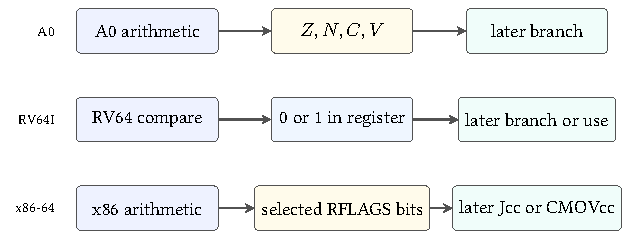
\includegraphics[width=0.92\textwidth]{figures/condition-shapes}
\caption{Selected ways to preserve a decision for later use. A0 and x86-64
write condition state; RV64I can write an explicit Boolean register.}
\figalt{Three rows show A0 arithmetic through ZNCV to a branch, RV64 compare through a zero-or-one register to later use, and x86 arithmetic through RFLAGS to a conditional instruction.}
\label{fig:condition-shapes}
\end{figure}

RV64I base ADD and SUB write the destination register but no x86-style
arithmetic flags. \code{slt rd,rs1,rs2} writes one when the signed reading of
\code{rs1} is less than that of \code{rs2}, otherwise zero. \code{sltu} uses
unsigned readings. Branch instructions can compare registers directly. These
rules come from the pinned unprivileged specification
\autocite{riscv2026unpriv}.

x86-64 selected ADD, SUB, and CMP forms update arithmetic status flags including
CF, ZF, SF, and OF. CF records the unsigned carry or borrow convention of the
selected operation; OF records signed overflow; ZF records zero; SF records
the result high bit. Later conditional forms interpret combinations of those
bits. The exact affected and undefined flags remain form-specific in Intel's
pinned instruction reference \autocite{intel2026sdm2}.

A0's four names resemble that x86 subset, but resemblance is not identity.
A0 deliberately defines one no-borrow polarity for subtraction and explicit
policies for logic and zero-count shifts. A relation must map predicates after
checking these definitions, not map letters because they look familiar.

\begin{sidebar}[title={Compare information, not storage shapes}]
An A0 condition bit, an RV64 zero-or-one register, an RV64 direct branch
predicate, and an x86-64 flag formula can represent the same decision. A
cross-machine relation should equate that decision on the declared states. It
need not invent identical condition registers on all three machines.
\end{sidebar}

\section{Carry chains turn condition state into data}

A word is often only one limb of a larger integer. Let a three-word unsigned
number use little-indexed limbs \(x_0,x_1,x_2\), each of width \(w\). Add
the low limbs, store result limb \(r_0\), and pass carry \(c_1\) into the
next addition. Continue until the high limb produces final carry \(c_3\).

\begin{figure}[htbp]
\centering
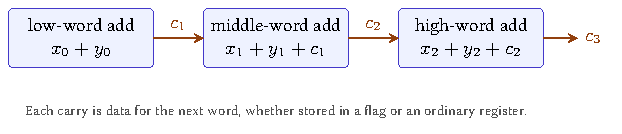
\includegraphics[width=0.88\textwidth]{figures/carry-chain-flow}
\caption{Multiprecision addition makes each carry a live input to the next
word. The storage location differs by ISA, but the mathematical recurrence is
the same.}
\figalt{Three word additions are connected left to right by carry values c1 and c2, with a final carry c3.}
\label{fig:carry-chain-flow}
\end{figure}

For limb \(i\), define the exact widened sum
\[
  s_i=\langle x_i\rangle_u+\langle y_i\rangle_u+c_i
     =c_{i+1}2^w+\langle r_i\rangle_u,
\]
with \(c_0=0\). Multiplying the equation for limb \(i\) by \(2^{wi}\) and
summing makes every internal carry cancel. The result is
\[
  X+Y=c_3 2^{3w}+R,
\]
where \(X,Y,R\) are the three-word unsigned readings. The local widened
identity therefore composes into a whole-number theorem.

This use makes condition liveness concrete. On a flag-based machine, an
instruction inserted between two limbs must not destroy the carry before the
next add-with-carry consumes it. On a machine without an architectural carry
flag, code may calculate the carry into an ordinary register and add it to the
next limb. The state shapes differ, but both proofs need the same recurrence
and must protect \(c_{i+1}\) across the intervening steps.

Signed multiprecision addition usually uses the same limb operations. Signed
overflow is judged at the high end from the full-width operand and result
signs, not by combining the per-limb overflow bits. Internal limbs are pieces
of one large representation; interpreting each as a separate signed integer
answers the wrong question.

\begin{proofkit}[title={Two-limb carry composition}]
Write the low identity as
\(x_0+y_0=c_1 2^w+r_0\) and the high identity as
\(x_1+y_1+c_1=c_2 2^w+r_1\). Multiply the high equation by \(2^w\) and add
the low equation. The terms \(c_1 2^w\) cancel from opposite sides, leaving
the exact two-limb sum with low limbs \(r_0,r_1\) and final carry \(c_2\).
\end{proofkit}

\section{Observed and unobserved conditions}

Consider two instruction sequences that always leave the same destination
word. One writes the correct conditions; the other leaves old conditions in
place. Under an observation of the destination alone, they can be equivalent.
Before a condition-reading branch, they need not be.

Take width-eight addition of \code{FF} and \code{01}. Both sequences store
\code{00}. The correct A0 conditions include \(Z=1,C=1,V=0\). If the faulty
sequence leaves \(C=0\), a later \code{branch.hs} chooses another path. The
destination-only claim and the flag-sensitive counterexample are both valid
because they use different observations and contexts.

The distinction determines legal optimization as well as good testing. A
compiler may replace an instruction with a flag-different sequence only when
the surrounding program cannot observe those flags before they are overwritten.
That fact can come from liveness analysis, a typed context, or a theorem whose
observation omits the condition state.

\begin{warning}[title={Dead conditions require evidence}]
Conditions are not unobservable merely because the current basic block does
not print them as outputs. A successor branch, conditional move, carry chain,
or surrounding context may read them. Prove that the relevant condition state
is dead or preserve it.
\end{warning}

The same reasoning applies to explicit Boolean registers. If an RV64 comparison
result is stored in a scratch register that the observation omits, changing it
may be harmless in one closed routine. If later code reads the register, the
difference is visible. Hidden versus explicit state changes the analysis tools,
not the need for a scope.

\subsection{Condition liveness is ordinary backward reasoning}

To decide whether a condition write matters, begin at the later use and reason
backward. A branch that reads \(Z\) makes the most recent reaching definition
of \(Z\) live. Earlier writes are dead if every path to the branch overwrites
\(Z\) first. If one path preserves an earlier value, that definition remains
live on that path. The same analysis applies separately to \(C\), \(V\), and
\(N\); treating the whole condition register as one indivisible value can be
safe but unnecessarily conservative.

Partial condition writes complicate the picture. If an instruction defines
\(Z,N\) while preserving \(C\), a later unsigned branch may depend on a carry
created several instructions earlier. If the architecture leaves a condition
undefined, a theorem cannot retain its old value unless the selected semantics
explicitly chooses that behavior. Undefined, preserved, and cleared are three
different policies.

An optimization proof can encode liveness as an observation boundary. Show
that both sequences agree on every location read before its next common
overwrite. Conditions absent from that set may differ. This local relation is
strong enough to justify replacement in the chosen context without making the
false global claim that the instruction sequences have identical complete
states.

\begin{example}[title={A carry survives an unrelated-looking operation}]
Suppose an addition creates a carry for the next limb. A candidate replacement
inserts a logical instruction before the add-with-carry. If that logical form
clears \(C\), the arithmetic destinations produced so far can still match,
yet the next limb differs. Backward liveness from the add-with-carry identifies
\(C\) as a required observation across the inserted instruction.
\end{example}

\section{How Axeyum can check the arithmetic layer}

The current Axeyum checkout provides reusable bit-vector and solver machinery
but not the A0 or real-ISA transition packages. The first implementation goal
for this chapter is a width-parametric arithmetic record containing the result
word and declared conditions. It should not begin with a full processor.

Implement pure functions for addition, subtraction, logic, and shifts. At
small widths, enumerate every input pair and compare the implementation with
independent mathematical definitions. At larger widths, ask a solver for a
counterexample to each equivalence: carry versus extended unsigned sum, signed
overflow versus the sign formula, subtraction no-borrow versus unsigned order,
and compare predicates versus signed or unsigned readings.

Every solver model should replay through the executable function. Negative
controls should invert carry, confuse carry with overflow, use \(N\) instead
of \(N\ne V\) for signed comparison, preserve a logic flag that A0 clears, and
mis-handle count zero. Each mutation has a small concrete witness, so a green
route that cannot reject it is not exercising the promised rule.

The first solver obligations can be small and independent of instruction
decoding. For arbitrary width-\(w\) bit vectors \(x,y\), build an extended
\((w+1)\)-bit sum by zero-extending both operands. Compare its low \(w\) bits
with the executable result and its high bit with executable carry. For signed
overflow, compare the executable bit with the high-bit Boolean formula. Ask
the solver for a state where either equality fails.

Subtraction needs its own obligation rather than reuse by name. Compare
executable no-borrow with unsigned \(x\geq y\), and executable signed
less-than with the signed bit-vector predicate. Shift checks quantify over a
raw count, derive A0's effective count, and split zero from nonzero before
stating the shifted-out-bit formula. These separate formulas make a failed
control diagnostic: a carry mutation should not be reported as an unrelated
signed-overflow failure.

At a teaching width, a census should retain counts as well as a pass bit. For
addition, partition every ordered pair by \((C,V)\), then retain one witness
from each nonempty class. Requiring all four classes prevents a checker from
passing only easy rows. A second census for subtraction should cover equality,
unsigned less-than, signed less-than, and the cases where the two orderings
disagree.

The future Python layer should expose these as explicit objects rather than a
single Boolean helper: an input domain, mathematical reference, executable
function, observation fields, enumerated census, solver query, replayed
witness, and semantic digest. The Rust layer should own the width-safe word
operations and serialized evidence checks. Python can assemble lessons and
display tables without becoming an unrecorded semantic authority.

\begin{goingdeeper}[title={From exhaustive rows to a universal formula}]
Width four has 256 ordered addition pairs. Exhaustive checking can classify
all of them by \(C\) and \(V\). The Boolean overflow proof covers every
positive width. Axeyum can connect the two: enumerate the teaching instance,
solve the general bit-vector negation at selected widths, and later reconstruct
a width-parametric theorem in a stronger kernel route. Keep those assurance
levels separate in the evidence record.
\end{goingdeeper}

Thin RV64I and x86-64 adapters come after the pure laws. The RV64 adapter maps
selected comparison results and arithmetic destinations. The x86 adapter maps
selected flags for exact operand widths and forms. An evidence manifest must
name the observation: destination only, selected conditions, or complete
in-scope state.

\section{Where the model stops}

This chapter treats integer words. It excludes floating-point exceptions,
saturation, packed lanes, decimal arithmetic, and multiprecision conventions
beyond a small carry-chain example. It does not claim that one flag policy
covers every x86-64 instruction form or optional RISC-V extension.

It also treats an instruction as an atomic state transition. Hardware may
compute condition information through internal circuits unlike these formulas.
The architectural theorem concerns the visible result, not the microarchitectural
route that produced it.

The reward for this restraint is a reusable core. A few finite-word identities
explain wraparound, comparisons, branches, and the legality of later program
transformations. The machine keeps only bits. A proof can still recover the
mathematical boundary those bits crossed.

The chapter's recurring method is deliberately uniform: widen when the exact
unsigned result matters, interpret high bits when signed range matters, and
name every condition-state policy that later code can observe. That method
scales from a four-bit teaching table to a multiprecision routine and from a
reader proof to a solver obligation without changing the meaning of the claim.

\section{Exercises}

\begin{enumerate}
\item \textbf{Execute.} For every ordered pair of width-two words, compute the
stored sum and A0 bits \(Z,N,C,V\). Group the rows by the four \((C,V)\)
combinations.

\item Give width-eight additions with carry but no signed overflow, signed
overflow but no carry, both conditions, and neither condition. Explain each
using mathematical ranges.

\item \textbf{Prove.} Prove that opposite-sign signed addition cannot overflow.
State the signed interval used by the proof.

\item Derive the Boolean high-bit formula for signed addition overflow and
check it on all four examples in Figure~\ref{fig:carry-overflow-quadrants}.

\item For width four, compute A0 subtraction conditions for
\code{0011-0101}, \code{0101-0011}, \code{0111-1111}, and
\code{1000-0001}.

\item Show with a concrete pair why \(N\) alone does not implement signed
less-than after subtraction. Show how \(N\ne V\) repairs the case.

\item Compare logical and arithmetic right shift of \code{10010000} by
counts 0, 1, 3, and 7 under A0. Include the last shifted-out bit.

\item \textbf{Break.} Replace signed overflow with carry in an A0 addition
implementation. Give the smallest-width counterexamples you can find in both
directions.

\item Construct two sequences with the same destination result but different
carry bits. Supply a suffix that observes the difference.

\item Explain how an RV64I \code{slt} result and an A0 \(N\ne V\) predicate
can represent the same signed comparison without identical machine states.

\item \textbf{Transfer.} State a relation between one selected x86-64 CMP
form and A0 \code{cmp}. Include operand width, subtraction polarity, mapped
conditions, program-counter relation, and excluded flags.

\item Design an Axeyum manifest for the width-four carry/overflow census.
Include the independent definition, row count, digest, replay check, and a
negative control.

\item Extend a destination-only arithmetic equivalence claim to a condition-
sensitive one. List the additional postconditions and tests required.
\end{enumerate}
